\documentclass[DaoFP]{subfiles}
\begin{document}
    \setcounter{chapter}{1}
    \chapter{Composition\\组合}

    \section{Composition\\组合}

    编程是关于组合(Composition)的。借用维特根斯坦(Wittgenstein)的话,可以说:“对于不能分解的东西,不应该谈论。”这不是一种禁止,而是一种事实陈述。研究、理解和描述的过程与分解的过程是一样的,我们的语言也反映了这一点。

    我们构建对象(Objects)和箭头(Arrows)词汇的原因正是为了表达组合的思想。

    给定一个从 $a$ 到 $b$ 的箭头 $f$ 和一个从 $b$ 到 $c$ 的箭头 $g$,它们的组合是一个直接从 $a$ 到 $c$ 的箭头。换句话说,如果有两个箭头,其中一个的目标与另一个的源相同,我们总是可以将它们组合起来得到第三个箭头。

    \[
        \begin{tikzcd}
            a
            \arrow[rr, bend left, "h"]
            \arrow[r, "f"']
            & b
            \arrow[r, "g"']
            & c
        \end{tikzcd}
    \]

    在数学中,我们用一个小圆圈来表示组合:
    \[h = g \circ f\]
    我们读作:“$h$ 是 $f$ 之后的 $g$。” 选择“之后”一词暗示了动作的时间顺序,这在大多数情况下是一种有用的直觉。

    组合的顺序可能看起来是反向的,但这是因为我们认为函数是在右边接受参数的。
    在 Haskell 中,我们用点号代替圆圈:
    \begin{haskell}
        h = g . f
    \end{haskell}
    这就是每个程序的简要概括。为了完成 \hask{h},我们将其分解为更简单的问题,即 \hask{f} 和 \hask{g}。这些问题可以进一步分解,依此类推。

    现在假设我们能够将 $g$ 自身分解为 $j \circ k$。我们有:
    \[h = (j \circ k) \circ f\]
    我们希望这个分解与以下分解相同:
    \[h = j \circ (k \circ f)\]
    我们希望能够说我们已经将 $h$ 分解为三个更简单的问题:
    \[h =  j \circ k \circ f\]
    而不必跟踪哪个分解是先进行的。这就是组合的\emph{结合性}(Associativity),从现在起我们将假设它。

    组合是箭头两种映射的来源,分别称为前置组合(Pre-composition)和后置组合(Post-composition)。

    当你\index{post-composition}\emph{后置组合}一个箭头 $h$ 和一个箭头 $f$ 时,它生成箭头 $f \circ h$(箭头 $f$ 是在箭头 $h$ \emph{之后} 应用的)。当然,你只能将 $h$ 与源是 $h$ 目标的箭头进行后置组合。通过 $f$ 的后置组合写作 $(f \circ -)$,为 $h$ 留下一个空位。老子会说,“后置组合的有用性来自于不存在的东西。”

    因此,一个箭头 $f \colon a \to b$ 诱导出箭头的映射 $(f \circ -)$,它将探测 $a$ 的箭头映射到探测 $b$ 的箭头。

    \[
        \begin{tikzcd}
            \node (a1) at (0, 2) {};
            \node (a2) at (-0.5, 2) {};
            \node (a3) at (0.5, 2) {};
            \node (aa) at (0.5, 1) {};
            \node(a) at (0, 0) {a};
            \draw[->, red] (a1) -- (a);
            \draw[->] (a2) -- (a);
            \draw[->, blue] (a3) -- (a);
            \node (b1) at (3+0, 2) {};
            \node (b2) at (3-0.5, 2) {};
            \node (b3) at (3+0.5, 2) {};
            \node (bb) at (2.5, 1) {};
            \node(b) at (3, 0) {b};
            \draw[->, red] (b1) -- (b);
            \draw[->] (b2) -- (b);
            \draw[->, blue] (b3) -- (b);
            \draw[->] (a) -- node[below]{f} (b);
            \draw[->, dashed] (aa) -- node[above]{(f \circ -)} (bb);
        \end{tikzcd}
    \]
    由于对象没有\emph{内部}结构,当我们说 $f$ 将 $a$ 转换为 $b$ 时,这正是我们所指的。

    后置组合让我们可以将焦点从一个对象转移到另一个对象。

    相对地,你可以通过 $f$ 进行\index{pre-composition}\emph{前置组合},或者应用 $(- \circ f)$ 到源自 $b$ 的箭头,将它们映射到源自 $a$ 的箭头(注意方向的变化)。

    \[
        \begin{tikzcd}
            \node (a1) at (0, -2) {};
            \node (a2) at (-0.5, -2) {};
            \node (a3) at (0.5, -2) {};
            \node (aa) at (0.5, -1) {};
            \node(a) at (0, 0) {a};
            \draw[<-, red] (a1) -- (a);
            \draw[<-] (a2) -- (a);
            \draw[<-, blue] (a3) -- (a);
            \node (b1) at (3+0, -2) {};
            \node (b2) at (3-0.5, -2) {};
            \node (b3) at (3+0.5, -2) {};
            \node (bb) at (2.5, -1) {};
            \node(b) at (3, 0) {b};
            \draw[<-, red] (b1) -- (b);
            \draw[<-] (b2) -- (b);
            \draw[<-, blue] (b3) -- (b);
            \draw[->] (a) -- node[above]{f} (b);
            \draw[->, dashed] (bb) -- node[below]{(- \circ f)} (aa);
        \end{tikzcd}
    \]

    前置组合让我们可以将视角从观察者 $b$ 转移到观察者 $a$。

    前置和后置组合是箭头的映射。由于箭头形成集合,这些映射是集合之间的\emph{函数}(Functions)。

    另一种看待前置和后置组合的方式是,它们是两个孔的组合运算符 $(- \circ -)$ 的部分应用的结果,其中我们可以用一个固定的箭头预填一个孔或另一个孔。

    在编程中,出射箭头被解释为从其源提取数据。入射箭头被解释为生成或构造目标。出射箭头定义接口,入射箭头定义构造器。

    对于 Haskell 程序员,以下是作为高阶函数的后置组合的实现:
    \begin{haskell}
        postCompWith :: (a -> b) -> (x -> a) -> (x -> b)
        postCompWith f = \h -> f . h
    \end{haskell}
    类似地,前置组合的实现如下:
    \begin{haskell}
        preCompWith :: (a -> b) -> (b -> x) -> (a -> x)
        preCompWith f = \h -> h . f
    \end{haskell}

    做以下练习来证明自己,焦点和视角的转换是可组合的。
    \begin{exercise}\label{ex-yoneda-composition}
    假设你有两个箭头,$f \colon a \to b$ 和 $g \colon b \to c$。它们的组合 $g \circ f$ 诱导出箭头的映射 $((g \circ f) \circ -)$。证明如果你先应用 $(f \circ -)$ 然后再应用 $(g \circ -)$,结果是相同的。符号表示为:
    \[((g \circ f) \circ -) = (g \circ -) \circ (f \circ -)\]

    提示:选择一个任意对象 $x$ 和一个箭头 $h \colon x \to a$,看看是否得到相同的结果。注意,这里的 $\circ$ 是多义词。在右侧,它表示两个后置组合之间的常规函数组合。
    \end{exercise}

    \begin{exercise}
        确信前一个练习中的组合是结合的。提示:从三个可组合的箭头开始。
    \end{exercise}

    \begin{exercise}
        证明前置组合 $(- \circ f)$ 是可组合的,但组合的顺序是反向的:
        \[(- \circ (g \circ f)) = (- \circ f) \circ (- \circ g) \]
    \end{exercise}

    \section{Function application\\函数应用}

    我们准备好写第一个程序了。有句谚语说:“千里之行,始于足下。”考虑从 $1$ 到 $b$ 的旅程。我们的一小步可以是从终端对象 $1$ 到某个 $a$ 的箭头。它是 $a$ 的一个元素。我们可以将其写为:
    \[1 \xrightarrow x a \]
    旅程的其余部分是箭头:
    \[a \xrightarrow f b\]
    这两个箭头是可组合的(它们共享对象 $a$ 作为中间对象),它们的组合是从 $1$ 到 $b$ 的箭头 $y$。换句话说,$y$ 是 $b$ 的一个\emph{元素}:

    \[
        \begin{tikzcd}
            1
            \arrow[rr, bend left, "y"]
            \arrow[r, "x"']
            & a
            \arrow[r, "f"']
            & b
        \end{tikzcd}
    \]
    我们可以将其写为:
    \[y = f \circ x \]

    我们使用 $f$ 将 $a$ 的一个\emph{元素}映射到 $b$ 的一个\emph{元素}。由于这是我们经常做的事情,我们称之为函数 $f$ 对 $x$ 的\emph{应用},并使用简写符号
    \[y = f x \]
    让我们将其翻译为 Haskell。我们从一个类型为 $a$ 的元素 $x$ 开始(简写为 \hask{x :: ()-> a})
    \begin{haskell}
        x :: a
    \end{haskell}
    我们将一个函数 $f$ 声明为从 $a$ 到 $b$ 的“箭头对象”的元素
    \begin{haskell}
        f :: a -> b
    \end{haskell}
    其中的理解(稍后将详细说明)是它对应于从 \hask{a} 到 \hask{b} 的箭头。结果是 $b$ 的一个元素
    \begin{haskell}
        y :: b
    \end{haskell}
    定义为:
    \begin{haskell}
        y = f x
    \end{haskell}
    我们称之为将函数应用于参数,但我们能够完全用函数组合来表达它。(注意:在其他编程语言中,函数应用需要使用括号,例如 \hask{y = f(x)}。)

    \section{Identity\\恒等}

    你可以将箭头视为表示变化:对象 $a$ 变为对象 $b$。一个回环的箭头表示对象自身的变化。但是,变化有它的对偶:没有变化,无为,或者用老子的话来说,\emph{无为}(Wu Wei)。

    每个对象都有一个特殊的箭头,称为恒等(Identity),它使对象保持不变。这意味着,当你将这个箭头与任何其他箭头组合时,无论是入射的还是出射的,你都会得到那个箭头。作为一种动作,恒等箭头什么都不做,也不需要时间。

    对象 $a$ 上的恒等箭头称为 $id_a$。因此,如果我们有一个箭头 $f \colon a \to b$,我们可以在任一侧与恒等箭头组合

    \[id_b \circ f = f = f \circ id_a \]
    或用图像表示:
    \[
        \begin{tikzcd}
            a
            \arrow[loop, "id_a"']
            \arrow[r, "f"]
            & b
            \arrow[loop, "id_b"']
        \end{tikzcd}
    \]

    我们可以轻松检查恒等箭头对元素的作用。让我们取一个元素 $x \colon 1 \to a$ 并将其与 $id_a$ 组合。结果是:
    \[id_a \circ x = x\]
    这意味着恒等箭头使元素保持不变。

    在 Haskell 中,我们使用相同的名称 \hask{id} 表示所有的恒等函数(我们不会用其作用的类型下标)。上面的方程式,它指定了 \hask{id} 对元素的作用,直接翻译为:
    \begin{haskell}
        id x = x
    \end{haskell}
    并且它成为了函数 \hask{id} 的定义。

    我们之前已经看到,初始对象和终端对象都有唯一的回环箭头。现在我们说,每个对象都有一个回环的恒等箭头。记住我们之前说过的关于唯一性的内容:如果你能找到两个这样的东西,那么它们一定是相等的。我们必须得出结论,我们之前提到的这些唯一的回环箭头必须是恒等箭头。我们现在可以标注这些图:

    \[
        \begin{tikzcd}
            \hask{Void}
            \arrow[loop, "id"']
        \end{tikzcd}
        \begin{tikzcd}
            \hask{()}
            \arrow[loop, "id"']
        \end{tikzcd}
    \]

    在逻辑中,恒等箭头对应于自明的真理。它是一个简单的证明,证明“如果 $a$ 为真,那么 $a$ 为真。”这也被称为\emph{恒等规则}(Identity Rule)。

    如果恒等什么都不做,那为什么我们还要关心它?想象你正在进行一趟旅行,组合了一些箭头,发现自己回到了起点。问题是:你做了什么,还是你浪费了时间?回答这个问题的唯一方法是将你的路径与恒等箭头进行比较。

    有些往返旅行会带来变化,而有些则不会。

    更重要的是,恒等箭头将允许我们比较对象。它们是同构(Isomorphism)定义的重要组成部分。

    \begin{exercise}\label{ex-yoneda-identity}
    $(id_a \circ -)$ 对终止于 $a$ 的箭头做了什么?$(- \circ id_a)$ 对源自 $a$ 的箭头做了什么?
    \end{exercise}

    \section{Monomorphisms\\单态射}

    考虑函数 \hask{even},它测试其输入是否能被 2 整除:
    \begin{haskell}
        even :: Int -> Bool
    \end{haskell}
    这是一个多对一的函数:所有偶数映射到 \hask{True},所有奇数映射到 \hask{False}。输入的大部分信息被丢弃了,我们只对其偶性感兴趣,而不是它的实际值。通过丢弃信息,我们得到了抽象\footnote{抽象(Abstract)字面意思是“抽离”。}。函数(以及后来的函子)体现了抽象。

    与此相反的是函数 \hask{injectBool}:
    \begin{haskell}
        injectBool :: Bool -> Int
        injectBool b = if b then 1 else 0
    \end{haskell}
    这个函数不会丢弃信息。你可以从它的结果中恢复它的参数。

    不会丢弃信息的函数也很有用:它们可以被认为是将其源注入到其目标中。你可以将源的类型想象为嵌入到目标中的一种\emph{形状}。在这里,我们将一个包含两个元素的 \hask{Bool} 形状嵌入到整数类型中。

    \[
        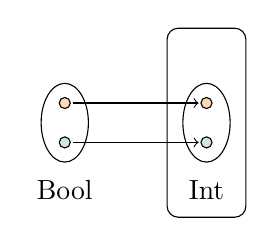
\begin{tikzpicture}
            \def\Xa{0};
            \def\Xb{1.8}
            \def\Y{0};
            \def\Yb{-0.85};
            \def\delta{0.1};

            \draw(\Xa, \Y) ellipse (0.3 and 0.5);
            % dots
            \draw (\Xa, \Y + 0.25) [fill=orange!30] circle (2pt);
            \draw (\Xa, \Y - 0.25) [fill=blue!50!green!20] circle (2pt);

            \draw [rounded corners] (\Xb - 0.5, \Y - 1.2) rectangle (\Xb + 0.5, \Y + 1.2) {};
            \draw(\Xb, \Y) ellipse (0.3 and 0.5);
            % dots
            \draw (\Xb, \Y + 0.25) [fill=orange!30] circle (2pt);
            \draw (\Xb, \Y - 0.25) [fill=blue!50!green!20] circle (2pt);
            % arrows
            \draw [->] (\Xa + \delta, \Y - 0.25) -- (\Xb - \delta, \Y - 0.25);
            \draw [->] (\Xa + \delta, \Y + 0.25) -- (\Xb - \delta, \Y + 0.25);
            % labels
            \node at (\Xa, \Yb) {Bool};
            \node at (\Xb, \Yb) {Int};
        \end{tikzpicture}
    \]

    单射(Injective Functions),或\index{injections}\emph{单射}(Injections),被定义为总是将不同的值分配给不同的参数。换句话说,它们不会将多个元素压缩为一个。

    这里有另一种稍微复杂的表达方式:单射仅当两个元素相等时才将它们映射为一个。

    我们可以将这个定义翻译为范畴语言,将“元素”替换为从终端对象来的箭头。我们会说,$f \colon a \to b$ 是单射的,如果对于任何一对全局元素 $x_1 \colon 1 \to a$ 和 $x_2 \colon 1 \to a$,有以下蕴涵成立:
    \[ f \circ x_1 = f \circ x_2 \implies x_1 = x_2 \]

    \[
        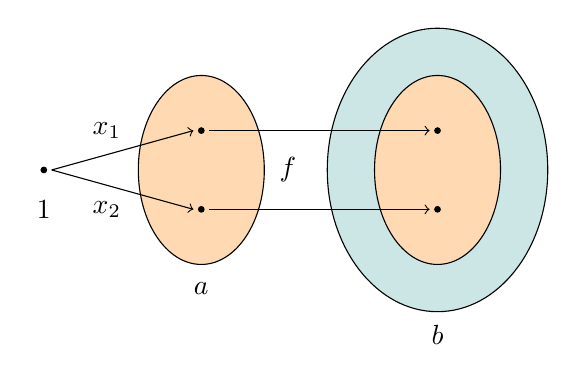
\begin{tikzpicture}
            \def\X{-2.0}
            \def\Xa{0};
            \def\Xmid{1.1};
            \def\Xb{3};
            \def\delta{0.1};

            \def\Ymid{0};
            \def\Ytip{-0.9};
            \def\Ybot{-1.5};
            \draw (\Xa , \Ymid)[fill=orange!30]  ellipse (0.8 and 1.2);
            \draw (\Xb, \Ymid)[fill=blue!50!green!20]   ellipse (1.4 and 1.8);
            \draw (\Xb , \Ymid) [fill=orange!30]  ellipse (0.8 and 1.2);
            % dots
            \filldraw (\X, \Ymid) circle (1pt);
            \filldraw (\Xa, \Ymid - 0.5) circle (1pt);
            \filldraw (\Xa, \Ymid + 0.5) circle (1pt);
            \filldraw (\Xb, \Ymid - 0.5) circle (1pt);
            \filldraw (\Xb, \Ymid + 0.5) circle (1pt);

            % arrows
            \draw [->] (\X + \delta, \Ymid) --  (\Xa - \delta, \Ymid + 0.5);
            \draw [->] (\X + \delta, \Ymid)  -- (\Xa - \delta, \Ymid - 0.5);
            \draw [->] (\Xa + \delta, \Ymid + 0.5) --  (\Xb - \delta, \Ymid + 0.5);
            \draw [->] (\Xa + \delta, \Ymid - 0.5)  -- (\Xb - \delta, \Ymid - 0.5);

            % labels
            \node at (\Xmid, \Ymid) { $f$ };
            \node at (\X + 0.8, \Ymid + 0.5) { $x_1$ };
            \node at (\X + 0.8, \Ymid - 0.5) { $x_2$ };
            \node at (\X, \Ymid - 0.5) {$1$};
            \node at (\Xa, \Ybot) {$a$};
            \node at (\Xb, \Ybot - 0.6) {$b$};

        \end{tikzpicture}
    \]

    这个定义的问题是,并非每个范畴都有一个终端对象。一个更好的定义将用任意形状替换全局元素。因此,单射的概念被推广为单态射(Monomorphism)。

    一个箭头 $f \colon a \to b$ 是\index{monomorphism}\emph{单态射}(Monomorphic)的,如果对于任何选择的对象 $c$ 和一对箭头 $g_1 \colon c \to a$ 和 $g_2 \colon c \to a$,有以下蕴涵成立:
    \[ f \circ g_1 = f \circ g_2 \implies g_1 = g_2 \]

    要证明箭头 $f \colon a \to b$ 不是单态射,只需找到一个反例:$a$ 中的两个不同形状,$f$ 将它们映射到 $b$ 中相同的形状。

    单态射或简称“单态”(Monos)通常用特殊的箭头表示,如 $a \hookrightarrow b$ 或 $a \rightarrowtail b$。

    在范畴论中,对象是不可分的,因此我们只能通过箭头谈论子对象。我们说,单态射 $a \hookrightarrow b$ 选择了 $b$ 中形状为 $a$ 的子对象。

    \begin{exercise}
        证明从终端对象来的任何箭头都是单态射。
    \end{exercise}

    \section{Epimorphisms\\满态射}

    函数 \hask{injectBool} 是单射(因此是单态射),但它仅覆盖了其目标的一小部分——在无穷多个整数中只有两个。
    \begin{haskell}
        injectBool :: Bool -> Int
        injectBool b = if b then 1 else 0
    \end{haskell}
    相比之下,函数 \hask{even} 覆盖了整个 \hask{Bool}(它可以生成 \hask{True} 和 \hask{False})。覆盖其整个目标的函数称为\index{surjection}\emph{满射}(Surjection)。

    为了推广单射,我们使用了额外的映射输入。为了推广满射,我们将使用映射输出。满射的范畴对应物称为满态射(Epimorphism)。

    一个箭头 $f \colon a \to b$ 是\index{epimorphism}\emph{满态射}(Epimorphism)的,如果对于任何选择的对象 $c$ 和一对箭头 $g_1 \colon b \to c$ 和 $g_2 \colon b \to c$,有以下蕴涵成立:
    \[ g_1 \circ f = g_2 \circ f \implies g_1 = g_2 \]
    相反,要证明 $f$ 不是满态射,只需选择一个对象 $c$ 和两个不同的箭头 $g_1$ 和 $g_2$,它们在与 $f$ 预组合时一致。

    为了深入理解这个定义,我们必须将映射输出可视化。正如映射到对象可以被认为是定义一种形状,映射出对象可以被认为是定义该对象的属性。

    当处理集合时,这一点很清楚,尤其是当目标集是有限时。你可以将目标集的一个元素视为定义一种颜色。源中的所有元素映射到该元素时都被“涂”上一种特定的颜色。例如,函数 \hask{even} 将所有偶数整数涂上 \hask{True} 的颜色,将所有奇数整数涂上 \hask{False} 的颜色。

    在满态射的定义中,我们有两个这样的映射,$g_1$ 和 $g_2$。假设它们之间仅有轻微差异。$b$ 的大部分被它们两者相似地涂上了颜色。

    \[
        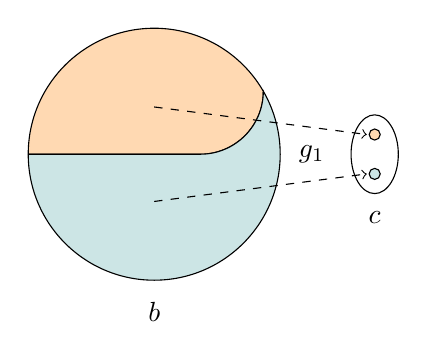
\begin{tikzpicture}
            \def\Xa{0};
            \def\Xmid{1.2};
            \def\Xb{3.2};
            \def\Xc{6};
            \def\delta{0.1};
            \def\d{0.3};
            \def\R{0.8};

            \def\Y{0};
            \def\Ybot{-2};

            \draw(\Xc, \Y) ellipse (0.3 and 0.5);
            % areas
            \draw [fill=orange!30] (\Xb - 2 * \R, \Y)
            arc[start angle=180, delta angle=-180+30, radius=2 * \R]
            arc[start angle=0, delta angle=-90, radius=\R]
            to (\Xb - 2 * \R, \Y);

            \draw [fill=blue!50!green!20]  (\Xb - 2 * \R, \Y)
            arc[start angle=-180, delta angle=180+30, radius=2 * \R]
            arc[start angle=0, end angle=-90, radius=\R]
            to (\Xb - 2 * \R, \Y);

            % dots
            \draw (\Xc, \Y + 0.25) [fill=orange!30] circle (2pt);
            \draw (\Xc, \Y - 0.25) [fill=blue!50!green!20] circle (2pt);

            % arrows
            \draw[->, dashed] (\Xb, \Y + 0.6) -- (\Xc - \delta, \Y + 0.25);
            \draw[->, dashed] (\Xb, \Y - 0.6) -- (\Xc - \delta, \Y - 0.25);
            % labels
            \node at (\Xc - 0.8, \Y) { $g_1$ };
            \node at (\Xb, \Ybot) {$b$};
            \node at (\Xc, \Y - 0.8) {$c$};
        \end{tikzpicture}
        \hspace{1cm}
        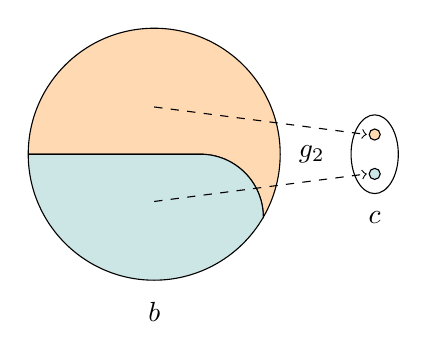
\begin{tikzpicture}

            \def\Xa{0};
            \def\Xmid{1.2};
            \def\Xb{3.2};
            \def\Xc{6};
            \def\delta{0.1};
            \def\d{0};
            \def\R{0.8};

            \def\Y{0};
            \def\Ybot{-2};

            \draw(\Xc, \Y) ellipse (0.3 and 0.5);
            % areas
            \draw [fill=orange!30] (\d + \Xb - 2 * \R, \Y)
            arc[start angle=180, delta angle=-180-30, radius=2 * \R]
            arc[start angle=0, delta angle=90, radius=\R]
            to (\d + \Xb - 2 * \R, \Y);

            \draw [fill=blue!50!green!20]  (\d + \Xb - 2 * \R, \Y)
            arc[start angle=-180, delta angle=180-30, radius=2 * \R]
            arc[start angle=0, end angle=90, radius=\R]
            to (\d + \Xb - 2 * \R, \Y);

            % dots
            \draw (\Xc, \Y + 0.25) [fill=orange!30] circle (2pt);
            \draw (\Xc, \Y - 0.25) [fill=blue!50!green!20] circle (2pt);

            % arrows
            \draw[->, dashed] (\Xb, \Y + 0.6) -- (\Xc - \delta, \Y + 0.25);
            \draw[->, dashed] (\Xb, \Y - 0.6) -- (\Xc - \delta, \Y - 0.25);
            % labels
            \node at (\Xc - 0.8, \Y) { $g_2$ };
            \node at (\Xb, \Ybot) {$b$};
            \node at (\Xc, \Y - 0.8) {$c$};
        \end{tikzpicture}
    \]

    如果 $f$ 不是满态射,可能它的像只覆盖了由 $g_1$ 和 $g_2$ 相似地涂上的部分。然后这两个箭头在与 $f$ 预组合时在 $a$ 上的表现一致,即使它们在整体上是不同的。

    \[
        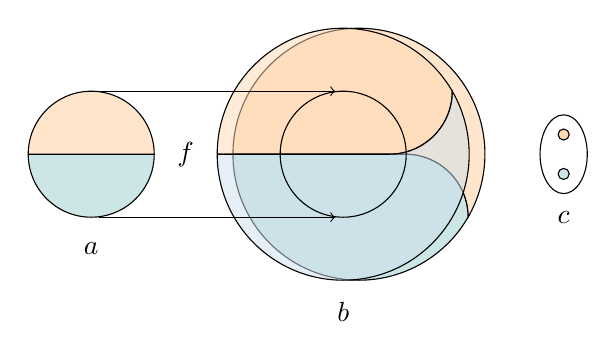
\begin{tikzpicture}
            \def\Xa{0};
            \def\Xmid{1.2};
            \def\Xb{3.2};
            \def\Xc{6};
            \def\delta{0.1};
            \def\d{0.2};
            \def\R{0.8};

            \def\Y{0};
            \def\Ymid{-1.2};
            \def\Ybot{-2};

            % \draw (\Xa , \Y)  circle ( \R);
            \draw [fill=blue!50!green!20] (\Xa - \R, \Y)
            arc[start angle = -180, delta angle = 180, radius = \R]
            to (\Xa - \R, \Y);
            \draw [fill=orange!20] (\Xa - \R, \Y)
            arc[start angle = -180, delta angle = -180, radius = \R]
            to (\Xa - \R, \Y);

            \draw(\Xc, \Y) ellipse (0.3 and 0.5);
            % area right
            \draw [fill=orange!20] (\d + \Xb - 2 * \R,  \Y)
            arc[start angle=180, delta angle=-180-30, radius=2 * \R]
            arc[start angle=0, delta angle=90, radius=\R]
            to (\d + \Xb - 2 * \R, \Y);

            \draw [fill=blue!50!green!20]  (\d + \Xb - 2 * \R, \Y)
            arc[start angle=-180, delta angle=180-30, radius=2 * \R]
            arc[start angle=0, end angle=90, radius=\R]
            to (\d + \Xb - 2 * \R, \Y);
            % area left
            \draw [fill=orange!30, fill opacity=0.5] (\Xb - 2 * \R, \Y)
            arc[start angle=180, delta angle=-180+30, radius=2 * \R]
            arc[start angle=0, delta angle=-90, radius=\R]
            to (\Xb - 2 * \R, \Y);

            \draw [fill=blue!60!green!20, fill opacity=0.5]  (\Xb - 2 * \R, \Y)
            arc[start angle=-180, delta angle=180+30, radius=2 * \R]
            arc[start angle=0, end angle=-90, radius=\R]
            to (\Xb - 2 * \R, \Y);

            \draw (\Xb , \Y)  circle ( \R);

            % dots
            \draw (\Xc, \Y + 0.25) [fill=orange!30] circle (2pt);
            \draw (\Xc, \Y - 0.25) [fill=blue!50!green!20] circle (2pt);

            %\filldraw (\Xb + \R + 0.7 * \R, \Y + 0.1)  circle (1pt);

            % arrows
            \draw [->] (\Xa + \delta, \Y + \R) --  (\Xb - \delta, \Y + \R);
            \draw [->] (\Xa + \delta, \Y - \R)  -- (\Xb - \delta, \Y - \R);

            % labels
            \node at (\Xmid, \Y) { $f$ };
            \node at (\Xa, \Ymid) {$a$};
            \node at (\Xb, \Ybot) {$b$};
            \node at (\Xc, \Y - 0.8) {$c$};

        \end{tikzpicture}
    \]
    当然,这只是一个插图。在实际范畴中是不能窥探对象内部的。

    满态射或简称“满态”(Epis)通常用特殊箭头表示,如 $a \twoheadrightarrow b$。

    在集合中,同时是单射和满射的函数称为双射(Bijection)。它在两个集合的元素之间提供了一个一对一的可逆映射。在范畴论中,这个角色由同构(Isomorphisms)扮演。然而,一般来说,并不是真的同时是单态射和满态射的箭头就是同构的。

    \begin{exercise}
        证明到终端对象的任何箭头都是满态射。
    \end{exercise}

\end{document}